%!TeX root=../Dissertation.tex
%!TeX bibfile=./introduction.bib
%!TeX bibfile=./synthesis.bib
%!TeX bibfile=./analysis.bib

\chapter{Introduction}
\section{Summary of the Current Situation}
\label{CurrentSituation}
Within computer networking, and computing as a whole, we tend to move through paradigms. Generally, there is a set way of doing things and eventually there are breakthroughs that shift that standard. One such paradigm is the use and reliance of Virtual Machines in the hosting of servers. As written by \citet{VirtualNetworkingInTheFuture}, ``Virtualization has rapidly become a go-to technology for increasing efficiency in the data center.''. Ameen and Hamo were right when they wrote this in 2013 and more and more server infrastructure has moved to virtualisation since. If we look at uptake of virtualised networking, servers and storage more recently, we see can see that virtualisation has become one of the de-facto solutions for server management. \citet{Spiceworks} found in ``The 2020 State of Virtualization Technology'' report that 92\% of the companies that they surveyed already used server virtualisation, with a further 5\%  planning on adopting it within two years of that date \citep{Spiceworks}. Some of the main reasons for this extremely high adoption are: savings in power and hardware (One physical machine can support multiple servers) and Logical Resource Consolidation \citep{LetsGetVirtual}. These savings however, don't come at no cost. One of the main stresses on any virtualised server infrastructure is the high resource usage that comes with hosting more than one server-based service on one physical machine. As server tasks become more strenuous, or when entirely new services need to be added to an already existing infrastructure, we can find that hardware (such as memory and CPU usage) becomes overwhelmed \citep{LetsGetVirtual}. As the tech world moves forward, the infrastructure that supports that tech within organisations needs to do so too. This is why we are starting to see a large number of organisations moving to cloud-based infrastructure, or taking the leap to invest in upgraded server hardware, that can withstand the large workloads required for some modern-day server loads. These solutions however, come with their own problems and negate the key reasons that these organisations moved to virtualisation in the first place. Cloud-based solutions, whilst being able to take the onus away from an organisations infrastructure team, can also result in costly hosting fees, not to mention the fact that cloud services often can't be used in place of some internal network components, such as DHCP and internal DNS servers. The other solution; upgrading hardware, again misses the mark and undermines the reasoning for why virtualisation was implemented in the first place. As already discussed, virtualisation is preferred because it can save money on costly server infrastructure. Instead of having to purchase (and power) several physical machines, you have one powerful machine that can support all the same services. When we reach the ceiling in terms of output from that sole machine, an upgrade seems inviable, but at this point, how much money was actually saved? Once you factor in the extra overhead that running a virtual machine introduces as a result of Virtual Machine and OS virtualisation resource usage (Figure \ref{fig:VirtualisationDiagram}), we start to see that Virtualisation might not be the perfect solution it once was.


\fbox{\parbox{\dimexpr\linewidth-2\fboxsep-2\fboxrule\relax}{\centering For reference only, Figure \ref{fig:VirtualisationDiagram} \\ 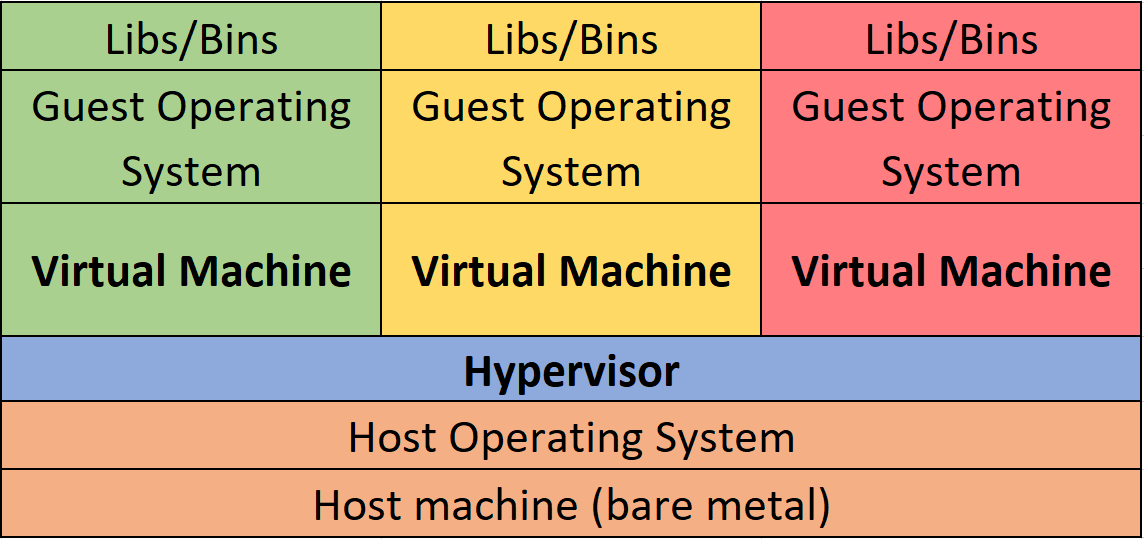
\includegraphics[width=0.9\textwidth]{./analysis/VMdiagram.PNG}}}

\section{A New Contender: Containers}
\label{IntroContainer}
One possible solution to this problem, is instead of upgrading hardware, organisations simply remove the Virtual Machine and virtualised OS components, along with their resource utilisation, whilst keeping the core functionality of the servers that they host intact, as shown in Figure \ref{fig:ContainerDiagram}. This is where containerisation comes into play. Containerisation, removes the need to virtualise a whole Operating System for each virtual machine, instead ingratiating with the host machine's Operating System directly, whilst keeping each container separated logically. These containers can still interface with real networks in much the same way that Virtual Machines do, but also reduce the overheads and the hardware resource utilisation dramatically. This allows SME's and other organisations currently using Virtualisation to squeeze more performance out of their already existing hardware without having to do costly upgrades to hardware.

\fbox{\parbox{\dimexpr\linewidth-2\fboxsep-2\fboxrule\relax}{\centering For reference only, Figure \ref{fig:ContainerDiagram} \\ \includegraphics[width=0.9\textwidth]{./analysis/Condiagram.PNG}}}

There has been a number of reports and published papers recently that demonstrate the improvements that containers offer over Virtual Machines for different use cases such as \citet{dua14} who found that Containers had a significant advantage over Virtual Machines in Platform as a Service environments. Another example of such findings is \citeauthor{joy15}'s ``Performance comparison Linux Containers and Virtual Machines'' (\citeyear{joy15}). This research found, as expected, that containers were much faster at processing requests than virtual machines. Where this research falls down however, is the range of data. Testing was done across a few areas, but is not all-encompassing of any specific area. Rather, it is a first look into the benefits of containers, without a real and solid recommendation on who should move to containers, and exactly what the benefits would be to any real-world systems.

There are countless more studies that could be mentioned here in regards to the `containerisation vs virtualisation' discussion, but the key finding around these studies tends to be that containers are better in doing a set task, but rarely is that task designed in a way that would test the real merit of containerisation within a real-world system. As a result, no one study appears to give a direct recommendation to anyone about moving to containers, and as a result, it seems we are figuratively `stuck' in this paradigm of virtualisation.

The research in this project report aims to contribute to this possible paradigm shift by making the case for containerised server solutions. Containers may not be the replacement for large-scale cloud solutions that some want it to be, but in cases where servers must still remain internal like with DHCP and internal DNS (as discussed in section \ref{CurrentSituation}), containerisation offers a way to gain massive performance improvements along with decreased hardware utilisation.

\section{Aims, Objectives, and How They Were Met}
The key aim of this report was to compare Virtualisation and Containerisation in a test environment that better represents a real-world server system.

 In order to do this, we set and then met a number of objectives. Firstly, we set out an analysis part, where we have discussed the current problem domain surrounding virtualisation, and why we need to find an alternative. Within this part we also explained the key differences between containerisation and virtualisation as this is very important to provide context to the research that is conducted in later parts.

As discussed in section \ref{IntroContainer} above, there is a lack of comparisons in this field that actually test real-world environments. As a result, the next step for this report was to carefully select both the hardware and software to be used in testing, and design an infrastructure topology that accurately reflects what could be a real-world internal server environment. Two separate systems were built, both using the exact same topology and configuration, but with one using a Container-based solution, and the other a Virtual-Machine solution. Then a total of four tests (with five data sources) were conducted across the entire topology. These tests were created in order to accurately evaluate the performance of both as a real-world server topology. This means the tests accurately measure parts of the topology that are actually important in those environments; instead of measuring just raw computing performance, we measured performance on the network, and the ability for each technology to perform common server-environment tasks, such as MySQL database OLTP \citep{oltpbenchmarking} and web server request latency. The Synthesis process was also conducted in a way that would allow us to pull information about the process of setting these systems up using our chosen tools. This information is important for our recommendation, as ease of use could be more important than performance for some end-users.

These tests then provided us with a large quantity of data that allowed us to compare the parallel performance of each server in either system. A detailed evaluation then followed, and with it we found that containers still hold up far better than virtual machines in a real server environment. As was planned, more detailed recommendations than seen from other similar studies were created. Through the method of creating the systems, we found that whilst creating both systems was relatively easy, there were some caveats in the process of using containers that hadn't previously been considered. This is exactly why matching research systems as closely as possible to real-world systems is so important. These findings are worked into the recommendations sufficiently.

There were of-course some planned limitations within the study that need to be addressed. Whilst we did look at areas other than just performance in our recommendation, the key and quantitative data was only performance oriented. There are other studies, such as \citeauthor{watanda19}'s “Emerging Trends, Techniques and Open Issues of Containerization: A Review” (\citeyear{watanda19}), which highlight security and isolation issues around containers, that are equally as important to the conversation around containers (Discussed further in section \ref{conclandreccoSecurity}). This was entirely out of the scope of our report though. The work that can be done in a one-person report has to be limited, and whilst further delving into an all-encompassing review of containerisation in server environments would have been something I would liked to have done, the scope of the report had to remain reasonable.

%Add more here to just finish off the introduction.



